%!TEX root = paper_main.tex
\section{Background}

\label{sec:threatmodel}

In this section, we define the threat model for a tracking attack on a BLE based mobile device. 
%
Following that we provide details on how extensive the threat is by exploring how all popular personal mobile devices are continuously and frequently transmitting BLE beacons.

%In this section we describe the threat model of location privacy attacks on
%BLE-enabled mobile devices. Then, we demonstrate how location privacy attacks
%are a significant threat today because popular mobile devices 
%continuously, and frequently, transmit BLE advertisements.

%Then, we explain why it may be possible to defeat BLE's built in anonymization
%techniques by physical-layer identity in the transmissions, that can defeat
%BLE's built-in anonymization techniques.

\subsection{Threat model: Passive fingerprinting of BLE mobile devices}
%
We consider an attacker that intends to detect when the target -- a particular user possessing the target mobile device --- is at a specific location (e.g. a room in a building or a crowded public place).
%
The attacker must possess a software-defined radio (SDR) to capture the raw \iq data of the BLE beacons transmitted by nearby mobile devices.
%
Even though a lot of SDR tools are expensive, we show in Section~\ref{sec:hadi:sdr} that a modest hobbyist-level SDR ($\sim$\$150) is sufficient for the attacker.
%

The attacker first captures a fingerprint of their target's mobile device.
%
They do so by getting close to them and capturing BLE beacons from their mobile device.
%
Then they use these BLE beacons to estimate unique physical-layer properties of the BLE transmitter hardware, such as CFO and \iq offset -- these define the fingerprint of the target mobile device.
%

Armed with the fingerprint of their target, the attacker sets up the receiver at the eventual attack location where they want to track the target.
%
The attacker captures beacon packets from all mobile devices at the location, estimates the physical-layer properties and compares it to the target fingerprint.
%
If the fingerprint matches, the attacker knows that the target is at the location.
%
The more frequently the BLE device transmits, the more likely the attacker is
to receive a transmission if a user passes by.  Also, the more accurate the
fingerprinting technique is, the better the attacker can differentiate the
target from other nearby devices.
%

\subsection{Extent of threat: Popular mobile devices are vulnerable} %{{{

Increasingly,  mobile devices are adding BLE beacons to
provide new features.
%
Most notably, during the COVID-19 pandemic, governments have installed software
on iPhones and Android phones to send constant BLE advertisements for digital
contact tracing: devices listen for nearby transmissions to determine if and
for how long another device was nearby.
%
Also, Apple and Microsoft operating systems have recently added BLE beaconing
to their devices for two inter-device communication features: lost device
tracking, and seamless user switching between devices (e.g., Apple's Continuity
Protocol, Microsoft's Universal Windows
Platform)~\cite{Iphonetracking_becker}.
%
Therefore, BLE beacons are now common on many mobile platforms, including:
phones, laptops, and smartwatches. 
 
%BLE beaconing presents a significant location privacy threat for
%the following reasons:
 
%\subsubsection*{BLE beaconing is widely deployed on mobile devices.}
%
%When mobile devices are running these applications, they need to constantly
%transmit BLE advertisements.

Fingerprinting and tracking a BLE device requires the device to act like a
tracking beacon: it must transmit continuously and frequently.
%
%Continuous beaconing creates a significant threat where users' devices are
%constantly emitting a signal that may be able to uniquely identify them.
%
We observed the BLE behavior of popular devices to determine if they transmit
continuously, and how frequently they transmit if they do.
%
Specifically, we isolated six popular devices in a Faraday
cage---ensuring they were the source of the transmissions---and we used an SDR sniffer
to collect all BLE advertisements (i.e., BLE beacons) transmitted on any of the three advertising channels. 
%
We observed the following:

\begin{table}
    \centering\small
    %\begin{minipage}{\textwidth}
      \captionsetup{justification=centering}
      \caption{BLE beaconing behavior of popular mobile devices.}
    \begin{tabular}{llc}
    \toprule
    \colname{Product} & \colname{OS} & \colname{\# of adverts/minute} \\
    \midrule
    iPhone 10 & iOS & 872 \\
    Thinkpad X1 Carbon & Windows & 864 \\
    MacBook Pro 2016 & OSX & 576 \\
    %Fitbit Alta HR & 54 \\
    Apple Watch 4 & iOS & 598 \\
    Google Pixel 5$^{*}$ & Android & 510 \\
    Bose QC35 & Unknown & 77 \\
    \bottomrule
    \multicolumn{3}{l}{\footnotesize{$^{*}$Only beacons with COVID-19 contact tracing enabled.}}

\end{tabular}

\begin{comment}
\begin{tabular}{lcc}
    \toprule
    \colname{Product}  & \colname{\# of adverts/minute} & \colname{Device state during test}\\
    \midrule
    iPhone 10 & 872 & Screen off and locked\\
    MacBook Pro 2016 & 576 & Screen off, \\
    Thinkpad X1 Carbon & 864 & Screen off, laptop on battery\\
    Fitbit Alta HR & 54 \\
    Apple Watch 4 & 598 \\
    Bose QC35 & 77 \\
    \bottomrule

\end{tabular}
\end{comment}

    
    \label{tab:beacon_rate}
    %\end{minipage}
\end{table}

\begin{enumerate}
\item \textbf{Mobile devices send BLE beacons continuously: }
%
We observed continuous BLE beaconing from all the six mobile devices shown in Table~\ref{tab:beacon_rate}.
%
%Mobile devices that transmit BLE beacons do so continuously, regardless
%of the user's activity on the device.
%
Even when all of these mobile devices have their screens off (e.g., they are in their user's pocket), they
continuously transmit BLE beacons. Indeed, this is a feature that is necessary for the proper function of the beacon applications such as contact tracing.
%
Continuous beaconing is a significant new threat compared to the behavior of other protocols on mobile devices that only transmit intermittently (e.g., periodic WiFi scanning).

\item \textbf{Mobile devices send hundreds of BLE beacons per minute:}

Table~\ref{tab:beacon_rate} also shows the average number of BLE beacons (i.e.,
BLE advertisements) we observed per minute from each device.
%
We observe that all of these devices transmit frequently---hundreds of packets
per minute---even when the device is otherwise idle (e.g., screen off).
%
%Even when these devices were in an idle state (i.e., screen off), they were
%still transmitting hundreds of beacons per minute.
%
Transmitting hundreds of advertisements per minute makes it feasible to produce a physical-layer fingerprint quickly: even if the device is in range of
the sniffer for a few seconds (Section~\ref{sec:results}).

%According to Bluetooth SIG, in 2018, an estimated $\sim$3.5 billion personal
%devices were shipped that contained Bluetooth chipsets, and more than 75\% of
%these chipsets were either BLE-only or were combo chips that included BLE
%capability~\cite{BTSIG_shipped_2019}.

%Also, an attacker may only need to sniff the devices for few seconds to have enough information to fingerprint them.
%}}}
\end{enumerate}


% Extra text {{{
\if 0
BLE advertisement packets transmitted by
nearby devices on one or more of the three BLE advertising channels (e.g., a
low-cost software defined radio such as Lime SDR). The attacker also has the
ability to store these captures to process them offline to extract the RF
fingerprint from the signals.  We consider our attacker to be a fully passive
observer. Namely, the attacker simply sniffs for BLE advertisements from nearby
devices to try to identify them.

\paragraph{1. Fingerprinting} The attacker must bring their capture device
close to the target at one given location. This will allow them to briefly
isolate that device's BLE advertisement packets in order to model that device's
RF fingerprint.  Once the attacker receives enough packets from that device to
produce a fingerprint, they can leave their receiver at one or more desired
locations and identify the target device whenever it appears. In
Section~\ref{sec:results:field} we demonstrate this can be done with only 100
packets which can be received in about one minute from most portable devices.  
\fi
%}}}

%}}}


\if 0
\subsection{BLE is difficult to fingerprint} %{{{
\label{sec:motivation:diff}

Although BLE poses a new and significant threat to the location privacy of
mobile device users, the protocol's design makes it extremely difficult to
obtain a reliable fingerprint of a device.
%
Specifically, the BLE protocol includes built-in mechanisms to prevent MAC
address fingerprinting, and the physical-layer signal is so simple that it is
difficult to produce a unique fingerprint.

\vspace{0.5em}
\noindent\textbf{MAC-Layer Fingerprinting:} 
%
At its most basic level, BLE's design frustrates MAC-layer fingerprinting.
%
Although BLE advertisements contain a full 6-byte MAC address that is unique to the
advertising device, the BLE protocol also has built-in cryptographic MAC randomization.
%
Fortunately, prior work found (and we confirmed) that mobile devices are
properly implementing BLE's MAC address randomization~\cite{Iphonetracking_becker,MACRandomizationfail_Martin}.
%
Namely, they found devices are following the BLE specification and periodically
(every 10--15 minutes) randomizing their MAC addresses~\cite{BTsigprivacy}.
%
However, this work also found that an attacker persistently following the target
device can track a device across MAC address changes by observing other fields
in the BLE beacon packet that were not reset properly after the MAC was
randomized.
%
This attack is extremely limited, it requires an attacker to
persistently follow a target to track it; therefore, if the attacker misses a
MAC randomization cycle it can no longer identify the target.

\begin{figure}
    \centering
    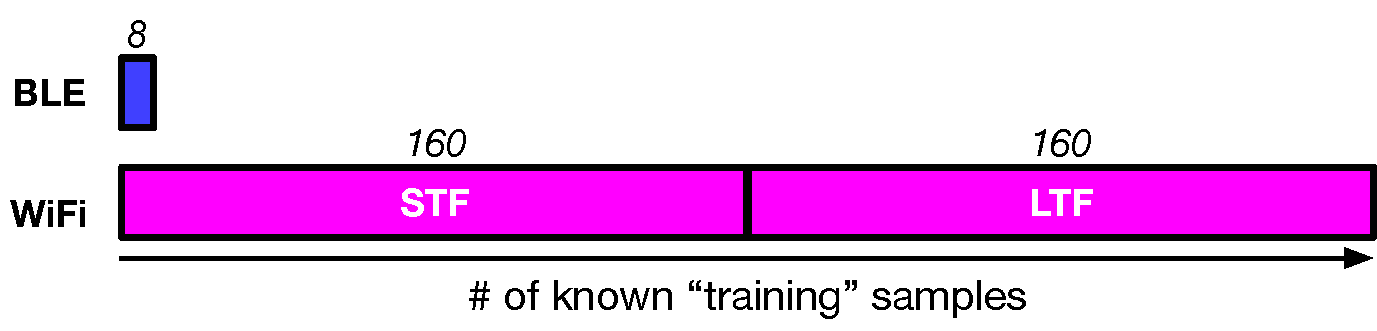
\includegraphics[width=\linewidth]{bletracking/plots/knownsamples}
    \caption{
      BLE packets have very few known samples for physical layer fingerprinting.
    \label{fig:2}
  }
\end{figure}

\vspace{0.5em} \noindent\textbf{Physical-layer fingerprinting:}
%
Physical layer fingerprinting is possible due to each radio having unique
hardware imperfections in its transmitter chain.
%
However, the design of BLE's physical layer is so simple that it is unlikely to
produce a unique physical-layer fingerprint. Also, even there were such a
fingerprint, it would be extremely difficult to extract that fingerprint from a
received BLE signal.
%
The reason is, BLE is an extremely low-energy protocol: BLE's physical-layer
signal is designed to require simple hardware to transmit and receive messages.
 
BLE signals are modulated basic Frequency Shift Keying (FSK) modulation. FSK
signals can be transmitted by a simple hardware phase-lock loop.
%
Such a simple transmitter will not have the complex hardware
impairments that have made it possible to fingerprint other mobile device protocols, namely WiFi~\cite{
vohuuusrp,
Brik_radiometric,
deviceID_kose}.
%
% Since these imperfections are
%caused by manufacturing variability, they can even produce a fingerprint for
%devices from the same make and model.
%
Additionally, BLE signals are so simple that they are difficult to recover a physical-layer fingerprint from.
%
%of a particular mobile
%device's radio is comparing known patterns in a signal received from that
%transmitter to the imperfect signal received from the transmitter.
%
Specifically, BLE transmissions do not require a significant number of known ``training''
samples for a receiver to use to correct for imperfections before decoding.
%  
These limitations make it difficult to apply existing physical-layer techniques~\cite{
vohuuusrp,
Brik_radiometric,
deviceID_kose,
Intrusion_hall,
suskitransient,
deeplearning_merchant,
lora_robyns,
gopalakrishnan2019robust}
to fingerprint BLE.
%
The problem is, these techniques have been developed for protocols, such as
WiFi, that require extremely accurate
corrections of impairments before they can be decoded.
%
%They require very accurate correction for imperfections in received signals
%before they can be successfully decoded.
%
Figure~\ref{fig:2} shows a comparison of the length of a typical
BLE beacon packet compared to a typical WiFi packet.
%
BLE packets only include 8 known symbols, whereas WiFi packets include 
a total of 320 known samples.

% Extra text {{{
\if 0
\paragraph{BLE Advertisement packets} BLE devices utilize advertisement packets
to indicate their presence to other devices in the vicinity. Advertisement
packets are short packets (at most 376 microseconds) which are frequently sent.
The packet length is shorter to save on energy and is typically 1/4 of the WiFi
packets. Advertisement packets include an 8-bit preamble, which is 10 $\times$
smaller compared to the WiFi preamble design. Furthermore, the packet consists
of a unique 48-bit identifier as advertising address (typically the hardware
MAC address of the radio), which is transmitted as part of the payload. Since
every packet contains the unique address, potential for tracking the device
became a concern. To alleviate this, Bluetooth SIG introduced address
randomization (as discussed in Section~\ref{sec:motivation}). Finally, the
complete advertising payload is appended with the CRC and is whitened or
scrambled. 

Hardware impairments in the transmitter chain which are caused by manufacturing
imperfections and tolerance, can make slight changes to the ideal signal that
should be sent by the device. Since these impairments are caused by
manufacturing imperfections, they are different even for the devices from the
same make and model. As a result, these hardware impairments can leave a unique
signature or fingerprint in the physical layer signal, that can be considered as
an identity for the device. Therefore, even though the MAC address changes
after a while, physical layer or radio frequency (RF) fingerprints remain the
same for a device which provides the attacker an opportunity to sniff the RF
fingerprints and identify the target at any time. Consequently, frequent
transmission of BLE packets can still cause a privacy threat even if MAC address
randomization is properly done. In this work, we aim to explore how practical
this attack could potentially be.
\fi
%}}}

\fi
